\chapter{Evaluation}
\label{cha:evaluation}

In this chapter, the performance of the trained behavioral cloning model (BCNet) is quantitatively and qualitatively compared to that of the expert control system. The evaluation is based on trajectory-level behavior analysis under controlled conditions, with specific attention to trajectory similarity, movement characteristics, and clustering structure.

\section{Experimental Setup}

To conduct a fair and objective evaluation, an overhead camera was installed above the arena to record the JetBot's movement during navigation tasks. The camera captured the complete trajectory of the robot in the $x$-$y$ plane for both the expert controller and the BCNet-driven controller.

Each trajectory represents a single run of the robot from start to completion of a predefined navigation task. The recorded video data was manually post-processed to extract discrete trajectory coordinates over time, resulting in a dataset suitable for further analysis and metric computation.

\section{First Difficulty}

To assess the similarity between the expert and neural network behaviors on the first difficulty level, several standard clustering and trajectory analysis metrics were applied. The two sets of trajectories generated by the expert and by the BCNet were treated as distinct clusters.

\subsection{Davies–Bouldin Index}

The \textbf{Davies–Bouldin Index (DBI)} is a widely-used clustering metric that evaluates intra-cluster similarity and inter-cluster separation \autocite{4766909}. A lower DBI indicates that the clusters are compact and well-separated. The DBI is calculated as:

\[
  \text{DBI} = \frac{1}{k} \sum_{i=1}^{k} \max_{j \ne i} \left( \frac{\sigma_i + \sigma_j}{d(c_i, c_j)} \right)
\]

Where $\sigma_i$ and $\sigma_j$ are the average distances of points in clusters $i$ and $j$ to their respective centroids, and $d(c_i, c_j)$ is the distance between cluster centroids. In this case, trajectory similarity was calculated using Dynamic Time Warping (DTW), which is more appropriate than Euclidean distance for comparing temporal sequences of varying length.

\textbf{Result:} The DBI for the expert and BCNet trajectories was \textbf{1.779}. The DBI of 1.779 suggests moderate overlap (values <1 indicate strong separation, >2 poor separation), implying that the model-generated trajectories share similar global structure with those of the expert, though some separation remains.

\subsection{Silhouette Score}

The \textbf{Silhouette Score} \autocite{kaufman2009finding} measures how similar an object is to its own cluster (cohesion) compared to other clusters (separation). It ranges from $-1$ to $1$, with higher values indicating better-defined clusters. It is defined as:

\[
  s(i) = \frac{b(i) - a(i)}{\max(a(i), b(i))}
\]

Where $a(i)$ is the mean intra-cluster distance and $b(i)$ is the mean nearest-cluster distance for sample $i$.

To better understand directional movement accuracy, silhouette scores were calculated independently for the $x$ and $y$ axes of the trajectories:

\begin{itemize}
  \item \textbf{X-Axis Silhouette Score:} $0.49$ — This relatively high score indicates that the BCNet has not succeeded in mimicking the forward-driving behavior of the expert.
  \item \textbf{Y-Axis Silhouette Score:} $0.32$ — This lower value reflects more precision in side-to-side movement, which is associated with steering and turning maneuvers.
\end{itemize}

The axis-wise silhouette scores reveal a key insight: BCNet replicates steering maneuvers (Y-axis) more faithfully than forward motion (X-axis). This aligns with the model's need to prioritize obstacle avoidance over speed regulation in this task.

The diagram of all of the trajectories made by both expert and trained model is shown in \autoref{fig:trajectory_overlay}. The axes represent the pixel coordinates on the video and do not correspond to actual coordinates in the real world.

\begin{figure}[htbp]
  \centering
  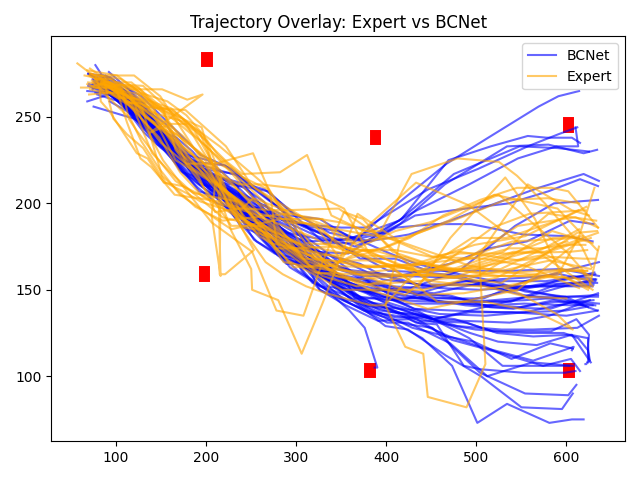
\includegraphics[width=0.6\textwidth]{Images/Evaluation/trajectory_overlay.png}
  \caption{Overlay of trajectories recorded from expert and BCNet-driven JetBot runs.}
  \label{fig:trajectory_overlay}
\end{figure}

\subsection{Mean Velocity Comparison}

Comparison between velocity profiles of the expert and the trained model is represented in \autoref{fig:velocity_profiles}. The average linear velocity of the JetBot throughout the whole trajectory was also analyzed:

\begin{itemize}
  \item \textbf{Mean velocity of BCNet:} $0.14$ m/s
  \item \textbf{Mean velocity of Expert:} $0.17$ m/s
\end{itemize}

This result shows that while the BCNet-driven JetBot was capable of navigating the environment, it tended to move more cautiously (i.e., slower) than the expert. This behavior is typical in behavioral cloning approaches, especially in cases of errors during training or a poorly constructed dataset \autocite{bühler2020drivingghostsbehavioralcloning}.

\begin{figure}[H]
  \centering
  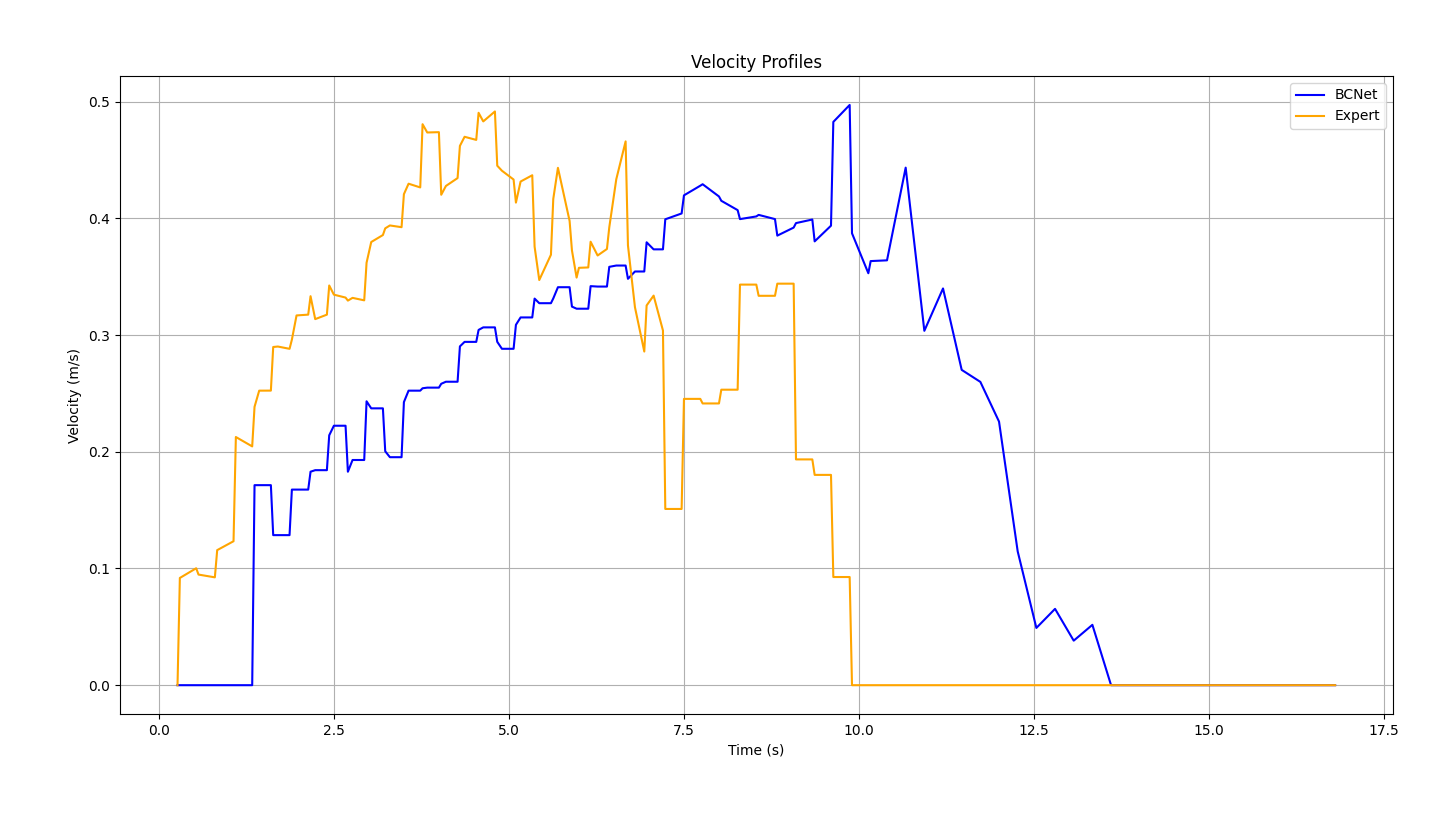
\includegraphics[width=0.8\textwidth]{Images/Evaluation/velocity_profiles.png}
  \caption{Mean velocity over time.}
  \label{fig:velocity_profiles}
\end{figure}

\subsection{Evaluation Metrics Summary}

The results presented in the \textit{Failure Rate per Obstacle – First Difficulty} table reveal a clear trend: the failure rate increases with the distance traveled by the JetBot. This is indicative of a distributional shift problem \autocite{codevilla2019exploring}, where the model's predictions become less reliable the further it moves from the initial conditions seen during training.

Two main causes of failure were observed. First, collisions often occurred due to physical constraints, such as the JetBot's external cables coming into contact with obstacles when navigating tight passages. Second, in some runs, the convolutional neural network produced control commands that led the JetBot into suboptimal trajectories, gradually evolving into states from which recovery became difficult. As the vehicle slowed down in these ambiguous regions, it eventually collided with an obstacle.

\begin{table}[H]
  \centering
  \caption{Failure Rate per Obstacle – First Difficulty}
  \begin{tabular}{|l|c|c|}
    \hline
    \textbf{Obstacle}      & \textbf{BCNet Failure Rate} & \textbf{Expert Failure Rate} \\
    \hline
    First Obstacle         & 0\%                         & 8\%                           \\
    Second Obstacle        & 2\%                         & 3\%                           \\
    Third Obstacle         & 27\%                        & 6\%                           \\
    \hline
  \end{tabular}
\end{table}

\begin{table}[H]
  \centering
  \caption{Trajectory Evaluation Metrics}
  \label{tab:evaluation_metrics}
  \begin{tabular}{|l|c|}
    \hline
    \textbf{Metric} & \textbf{Value} \\
    \hline
    Davies–Bouldin Index & 1.779 \\
    Silhouette Score (X-axis) & 0.49 \\
    Silhouette Score (Y-axis) & 0.32 \\
    Mean Velocity (BCNet) & 0.14 m/s \\
    Mean Velocity (Expert) & 0.17 m/s \\
    \hline
  \end{tabular}
\end{table}

\section{Second Difficulty}

In the second difficulty level, the model was tested in a modified environment where both the initial position of the JetBot and the locations of obstacles were varied. Although the BCNet-controlled JetBot was still capable of producing valid control commands and moving through the arena, it failed to complete any runs according to task requirements, resulting in a 0\% success rate.

Experiment results show that the model did not internalize the general concept of maneuvering between obstacles. In many cases, the JetBot traversed the arena in seemingly valid paths but deviated from the intended corridor, often leading to collisions. Most failures occurred upon approaching the second obstacle, where the JetBot was unable to perform the necessary maneuvering.
